\documentclass{ltjsarticle}
\usepackage{url}
\usepackage{graphicx}

\begin{document}
\begin{titlepage}
    \title{JSONファイルの記法}
    \author{谷口 陽音}
    \date{令和5年7月21日発行}
    \maketitle
\end{titlepage}
\section{はじめに}
テスト範囲まとめページを作成するのにあたり、一人で全データを入力するのは大変である。\\
そこで、はじめてでも書きやすいJSONというフォーマットでデータを入力できるようにしたため、各教科Google Forms入力担当者に教科ごとのテスト範囲入力を頼みたい。\\
しかし、JSONなんて書いたことない人が大半だと思うため、今回についてはこのマニュアルに沿って進めればできるようにしてある。
\section{準備}
\subsection{GitHubアカウント}
本プロジェクトのWebサイトは「GitHub Pages」というサービスを用いて運用している。\\
そこで、変更等を行うときにはGitHubアカウントが必要である。\\
GitHubアカウントはI1の実習でも使用するため、今回はI1実習の作成ルールに則って説明する。
GutHubアカウントを持っている人は
\subsection{GitHubアカウントの作成}
以下の手順で進める。
\begin{enumerate}
    \item \url{https://github.com}にアクセスする。
    \item 右上の「Sign Up」を選択(図\ref{github_top})
    \begin{figure}[htpb]
        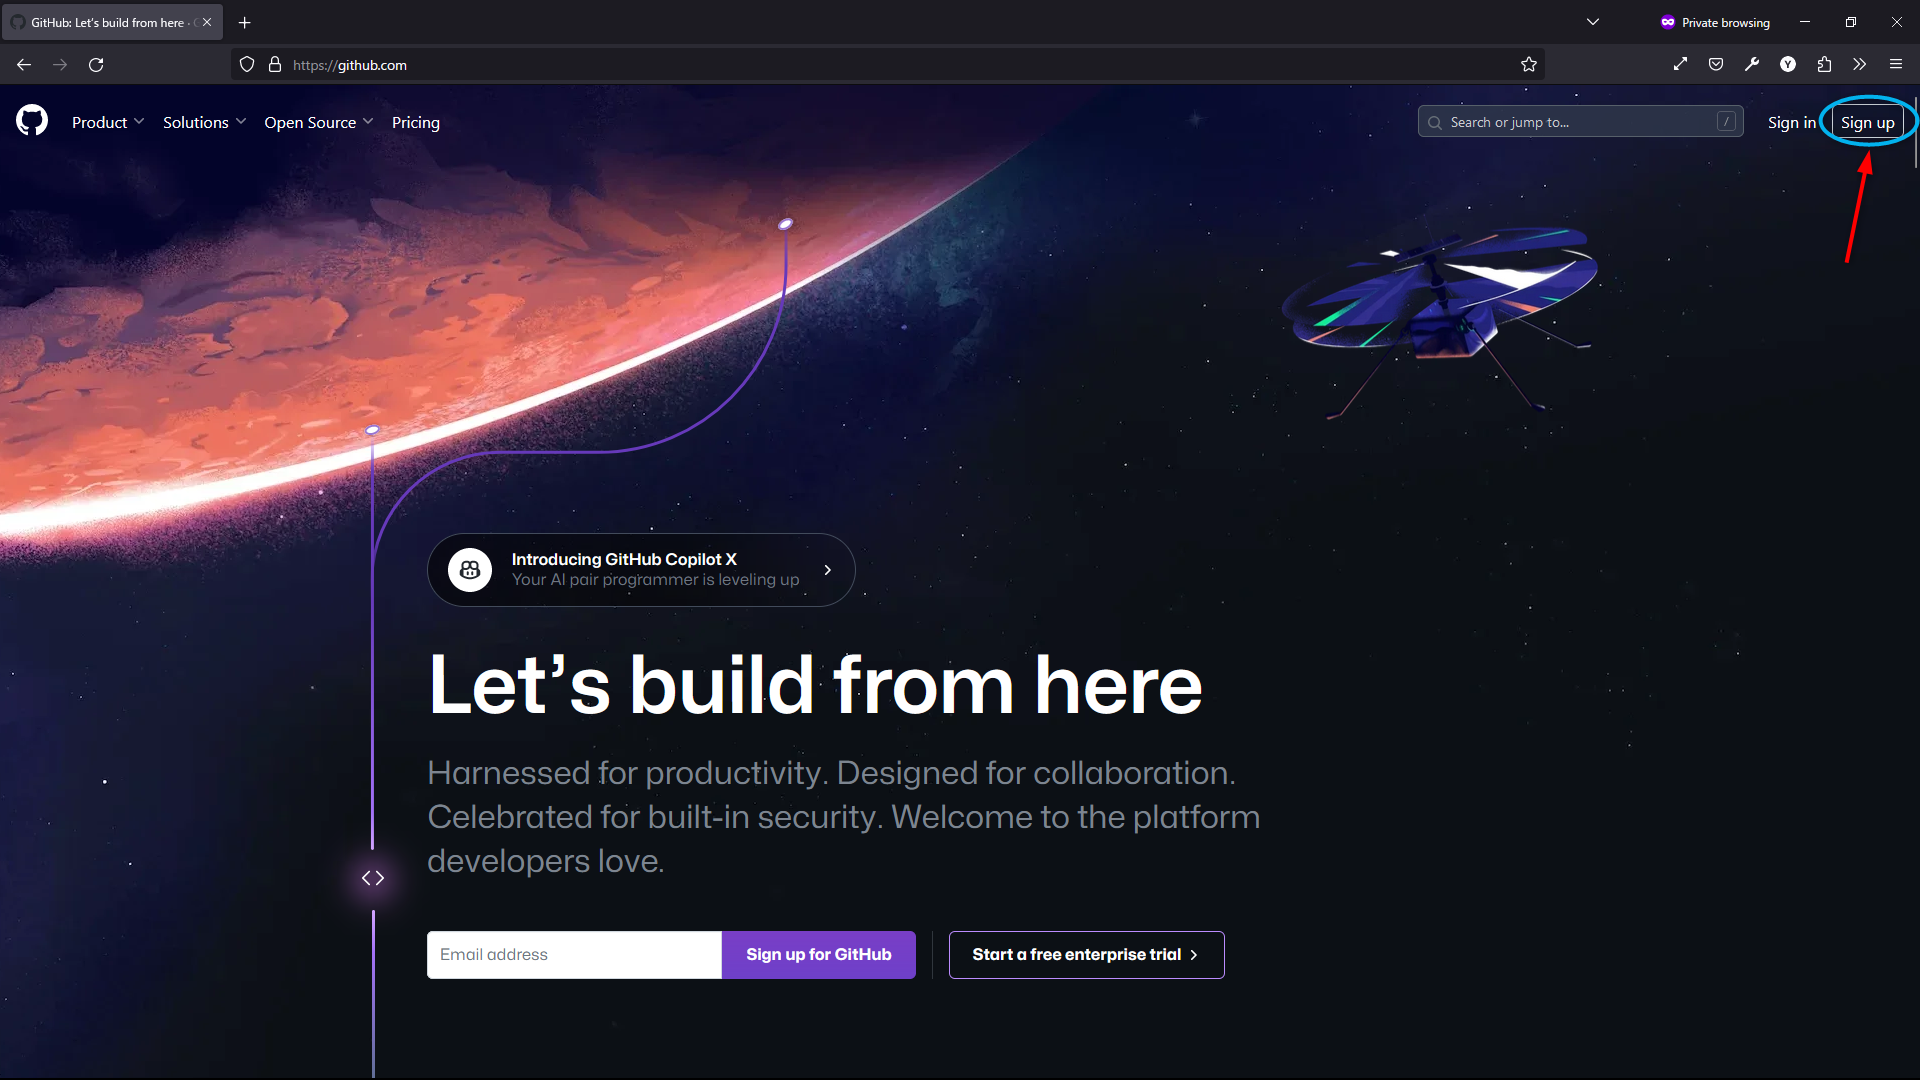
\includegraphics[width=15cm]{pictures/github_top.png}
        \caption{手順2}\label{github_top}
    \end{figure}
\end{enumerate}
\begin{figure}
    
\end{figure}
\end{document}